\section{Antennen}
\subsection{Antennen-Charakterisierung}
\begin{tabular}{ll}
\parbox{6cm}{
    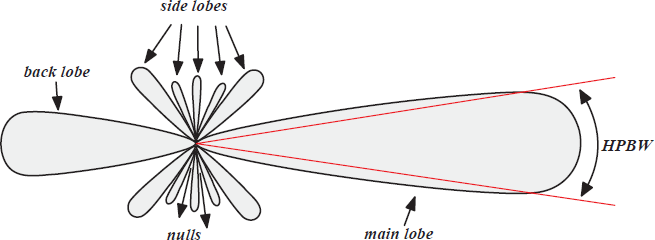
\includegraphics[width=6cm]{../MobKom2/bilder/antennas-radiation-pattern.png}}
& \parbox{12cm}{
\begin{liste}
	    \item Reziprozit�t: Charakteristiken der Antennen bleiben gleich, egal ob Antenne
	    als Sender oder Empf�nger gebraucht wird.
	    \item Radiation Pattern (Richtcharakteristik): 
	    \begin{liste}
		    \item {\em Half-power beamwidth} (kurz {\em beamwidth} oder HPBW): Winkel
		    zwischen beiden half-power Punkten in der main lobe.
		    \item {\em Front-back ratio}: Verh�ltnis zwischen Peak Amplituden der main
		    und back lobe.
		    \item {\em Sidelobe level}: Verh�ltnis der gr�sste Amplitude der side
		    lobe und dem peak der main lobe.
	    \end{liste}
	\end{liste}
	}
\end{tabular}\\
\begin{liste}
    \item Antennenfl�che (keine physikalische Interpretation): 
        $P = AS; \qquad A = \frac{\lambda^2 G}{4\pi} \quad G_{\text{dB}} = 10
        \log\left(\frac{4A\pi}{\lambda^2}\right)$
    \item Effektive Antennenl�nge: 
    $V= E \frac{l_{\text{eff}}}2 = \sqrt{\frac{|E|^2AR}{120\pi \Omega}}$
    $;\qquad$ $l_{\text{eff}} = \sqrt{\frac{AR}{30\pi \Omega}}$
    \item Antennenfaktor: $k = \frac{E}{V} = 20 \log
    f_{\text{MHz}}-29.78-G_{\text{dBi}}$
    \item Polarisation: Vertikal, horizontal; Recht-Hand (RHCP)/
    Link-Hand Zirkular (LHCP): Definition schwierig 
    \item Antenneneffizienz: $\eta = \frac{R_{\text{rad}}}{R_{\text{rad}} +
    R_{\text{loss}}}$
    \item Antennnegewinn (Gain): $G=\eta \cdot D$ ($D$ = maximale Direktivit�t)
    \item Bandbreite: Bereich, wo $G < 3dB$ bzw. VSWR $< 2:1$
    \item Einheiten: $\underbrace{0dBd}_{\text{\tiny{G von $\lambda/2$-Dipol}}}
    = \underbrace{2.15dBi}_{\text{\tiny{G von isotropischer Antenne}}}$
\end{liste}

\subsection{Antennentypen }
\subsubsection{�bersicht }
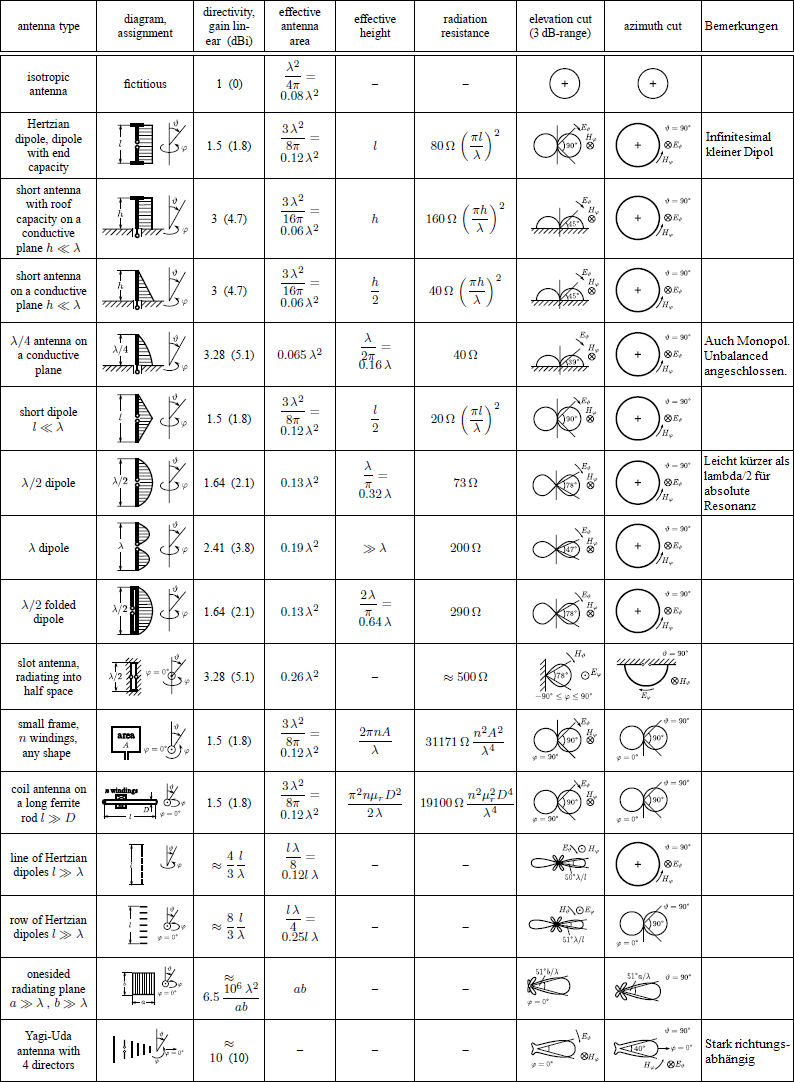
\includegraphics[angle=90,width=19cm]{../MobKom2/bilder/antennas-overview.png}

\subsubsection{Weitere Antennentypen }
\begin{tabular}{ll}
\parbox{11cm}{
    \textbf{Logarithmisch Periodische Antenne (LogPer):} \\
    �hnlich wie
    Yagi-Antenne, aber ausgerichtet auf hohe Bandbreite .\\
    
    
    \textbf{Loop-Antenne:} \\
    Ineffizient, daf�r kleiner Platzverbrauch.
    Herstellung als viereckige Metallstreifenloops oder als PCB.\\
    
    
    \textbf{Patch- bzw. Microstrip-Antenne (rechts):}\\
    V.a. in GPS und mobilen Ger�ten benutzt. Quadratischer oder runder Patch
    �ber Groundplane. $W = \lambda/2 \qquad L \approx 0.49
    \frac{\lambda}{\sqrt{\epsilon_r}}$ 
    }
& \parbox{8cm}{
    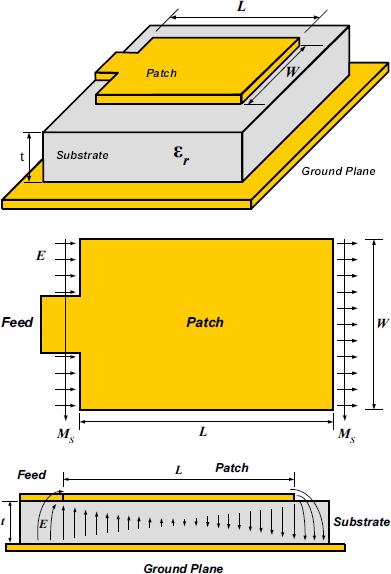
\includegraphics[width=5cm]{../MobKom2/bilder/antennas-patch.png}
    }
\end{tabular}




\subsection{Smart Antennas}

\begin{minipage}{9cm}
\begin{minipage}{4.5cm}
$$ \swarrow $$
$$ \text{Switched Beam:} $$
$$\text{Wechsel zwischen einer begrenzten}$$ 
$$\text{Anzahl an Pattern/Richtungen}$$
\end{minipage}
\begin{minipage}{4.5cm}
$$ \searrow $$
$$\text{adaptive Arrays:}$$
$$\text{zB. Beamforming}$$
\end{minipage}
\end{minipage}
\begin{minipage}{9cm}
\subsubsection{Einheiten}
$\vec{x_n}:Antenna Position$ \\
$k=\frac{2\pi}{\lambda}=\frac{2\pi}{Wellenl�nge}$\\
$\vec{y}: Receiver Position$\\
$\Delta\varphi=-k|\vec{x_n}-\vec{y}|$\\
$g(\vec{y})=
\sum\limits_{n=0}^{N-1}\omega_n g_n(\Phi)
e^{-j\Delta\varphi}=\sum\limits_{n=0}^{N-1}\omega_n g_n(\Phi)
e^{-jk|\vec{x_n}-\vec{y}|}$\\
$g=komplexes Empfangsignal$\\
$\omega_n=komplexe Amplitude von N-ten Antenne$\\
$g_n=Ausrichtung n-Antenne$\\
\textbf{Voraussetzung}\\
$|\vec{x_n}-\vec{y}|$ sind alle �hnlich zueinander $\Rightarrow$ FernFeld
\end{minipage}


\subsubsection{Linear Phase Array}
\begin{minipage}{8cm}
    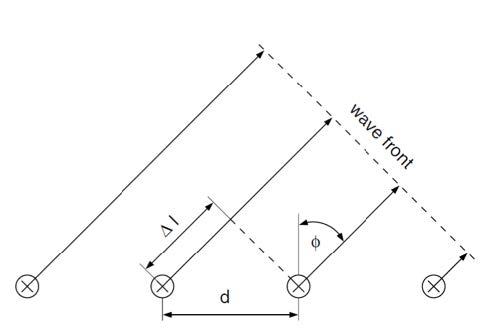
\includegraphics[width=8cm]{./bilder/LinearPhasedArray.jpg}
\end{minipage}
\begin{minipage}{9cm}
$\Delta\varphi=-k n d \sin(\Phi)=-k n \Delta l$\\
$g(\Phi)= \sum\omega_n g_n(\Phi) e^{-jknd\sin(\Phi)}$\\
wenn alle $\Phi_n$ gleich sind ($g_n(\Phi)=g_e(\Phi)$) und \\
$g_e$ auf 1 normiert $\Rightarrow$ $g_g(\Phi)=\sum \omega_n
e^{-jknd\sin(\Phi)}\\
 \Rightarrow$ entspricht der diskrete Fouriertransformation\\

\end{minipage}\\
Es gibt so etwas wie ein Niques Theorem:\\
$d \leq \frac{\lambda}{2}$; Wenn dieses eingehalten wird entstehen keine Side
Loops, welche einen Teil der Energie von der Maink�ule verbraucht\\

\subsubsection{Brodside Array}
$\omega_n =  \omega_0 \forall n$\\
$|g(\Phi)|=|\omega_0| |\frac{\sin(\frac{1}{2} N k d
sin(\Phi))}{sin(\frac{1}{2} k d sin(\Phi))}|$\\
Falls Niques Theorem nicht erf�llt wird:
$B\approx 2\Phi_Z=2\sin^{-1}(\frac{\lambda}{N d}) \approx \frac{2\lambda}{L}$\\
$L=d(N-1)$\\
Maximalstellen: $k d \sin(\Phi_p)=0 \Rightarrow \Phi_p = 0$\\
Nullstellen:    $\frac{1}{2} N k d \sin(\Phi_N)= \pi \Rightarrow
\sin(\Phi_N)=\frac{\lambda}{N d}$\\


